% SOICT 2026 submission — Springer CCIS format (single-blind: keep author names).
% Requires the Springer LNCS/CCIS class `llncs.cls` + `splncs04.bst` from
% https://soict.org/wp-content/uploads/2025/09/Latex-Template-for-Springer.zip
% Max 12 pages excluding references. Figure: convert docs/paper/diagrams/soict_harlstmgat.svg -> PDF.
\documentclass[runningheads]{llncs}
\usepackage{graphicx}
\graphicspath{{diagrams/}}   % figure lives in docs/paper/diagrams/ (do NOT add ./ — collides with output pdf)
\usepackage{booktabs}
\usepackage{amsmath}
\usepackage[T1]{fontenc}

\begin{document}

\title{Multi-Horizon Stock Volatility Forecasting}

\author{Author One\inst{1} \and Author Two\inst{1}}
\authorrunning{Multi-Horizon Volatility Forecasting}
\institute{Affiliation, City, Country \\ \email{\{author1,author2\}@example.edu}}

\maketitle

\begin{abstract}
We evaluate whether a deep sequence model or a cross-sectional graph-attention branch changes multi-horizon
daily Parkinson-variance forecasts relative to a linear Heterogeneous Autoregressive model, extended to five features (HAR-X), on the
Vietnamese equity market --- VN30 and VN100 --- under panel-correct inference.
Three models share the same five node features: a linear HAR-X, a
five-feature LSTM, and a five-feature LSTM+GAT (directed volume$\to$Parkinson Top-5 weighted two-hop
attention). For the learned models we report the mean (and standard deviation) over five training seeds ---
the mean of the seed-level metrics, not the metric of a seed-averaged ensemble. We report five metrics (MSE,
RMSE, MAE, QLIKE, $R^2$) with equal weight and assess significance with the date-clustered Diebold--Mariano
(DM) test on the five-seed ensemble forecast; predictions are floored at $10^{-2}$ times the per-node training
mean. The primary target is short-term (horizons $h\in\{1,5\}$); $h\in\{10,22\}$ are an extended study. HAR-X
has the lowest QLIKE at every horizon on both panels, and no learned model has a significantly lower QLIKE than
HAR-X at any horizon (date-clustered DM, $p\ge0.05$). At VN100 the deep models have the lowest MAE at $h1$
(LSTM vs HAR-X, $p<0.001$), and the LSTM+GAT has a significantly lower QLIKE than the no-graph LSTM at VN30
$h1$, VN100 $h1$ and VN100 $h5$, but not at VN30 $h5$ or the longer horizons. The per-seed QLIKE standard
deviation of the learned models (about $0.02$--$0.07$) is comparable to these graph-vs-LSTM differences, so the
graph effect is an ensemble-level effect within seed noise. At $h10$ and $h22$ HAR-X has the lowest MSE, RMSE,
QLIKE and $R^2$. The ranking is metric- and horizon-dependent, so all five metrics are reported with equal
weight. Methodologically, a naive per-observation DM test on this cross-sectionally dependent panel overstates
significance by roughly the square root of the number of stocks.
\keywords{Volatility forecasting \and HAR \and LSTM \and Graph Attention Network \and Diebold--Mariano.}
\end{abstract}

\section{Introduction}
Daily volatility forecasting underpins risk management, position sizing and derivative pricing. The HAR model
of Corsi~\cite{corsi2009} is a linear benchmark: a few OLS coefficients on daily, weekly and monthly
aggregates of realized volatility capture much of the long-memory structure. Deep sequence models and graph
neural networks are frequently proposed to capture nonlinear temporal dynamics and cross-sectional spillovers,
and the evidence that they beat HAR out of sample is mixed; positive claims are often confounded by
data-design choices, such as a common-date intersection that discards most of the panel or a naive
significance test on cross-sectionally dependent data.

This paper measures, under a single panel-correct evaluation on the Vietnamese equity market, whether the
temporal nonlinearity or the cross-sectional graph changes the forecast relative to a linear HAR-X. We ask: (1)
Does a deep temporal LSTM over the shared feature set change the out-of-sample forecast relative to the linear
HAR-X, and at which horizons and metrics? (2) Does a cross-sectional Graph Attention Network branch --- here a
directed volume$\to$Parkinson weighted graph --- change the forecast relative to the same-feature no-graph
LSTM? To answer these we use a \emph{masked panel}: rather than intersecting to the dates on
which every ticker is present, we keep the union of trading dates with node and target masks for tickers not
yet listed on a given date, so late-listed tickers are included without dropping whole dates and every model
--- including the graph model --- is trained and evaluated on the same panel with the same five features.

Our contributions are: (i) a multi-horizon benchmark on the masked VN30/VN100 panel that holds
the feature set and the data design fixed across HAR-X, an LSTM and an LSTM+GAT, so any difference is
attributable to a single component; (ii) per-horizon results on all five metrics (seed mean and standard
deviation) with the date-clustered DM test --- HAR-X has the lowest QLIKE at every horizon on both panels, with
no learned model significantly lower at any horizon, the deep models have the lowest short-horizon MAE on
VN100, and the LSTM+GAT has a significantly lower QLIKE than the no-graph LSTM at VN30 $h1$, VN100 $h1$ and
VN100 $h5$ (but not VN30 $h5$ or $h10$/$h22$), a difference of the same order as the learned models' per-seed
QLIKE dispersion; and (iii) a methodological contribution --- the
date-clustered DM test, since a naive per-observation test overstates significance by roughly the square root of the number of stocks. Every number is taken from a stored results file.

\section{Related Work}
\textbf{HAR and classical models.} HAR~\cite{corsi2009} approximates the long memory of realized volatility
with a daily/weekly/monthly cascade; recent work reports that rolling-window and specification choices, rather
than model class, often account for measured differences from HAR~\cite{audrino2025}. HARQ~\cite{harq2016}
exploits measurement error, and GARCH-family models remain standard conditional-variance benchmarks. We use
HAR-X as the linear baseline and GARCH(1,1) as a classical benchmark. \textbf{Deep and graph models.} LSTMs~\cite{lstm1997} are widely applied to
financial series, and graph neural networks model cross-asset spillovers, e.g.\ Graph Attention
Networks~\cite{gat2018}, multivariate realized-volatility GNNs~\cite{chen2022} and spillover-aware GNN-HAR
hybrids~\cite{gnnhar2025}; reported effects vary across studies and data designs. Volatility spillover
measurement has a long econometric tradition~\cite{dy2012}. \textbf{Graph construction.} Our graph uses a
directed volume$\to$Parkinson relation (each node attends to its Top-5 volume-shock leaders, edge-weighted,
over two hops), motivated by volume leading volatility. \textbf{Evaluation.} Volatility is latent, so we use
the proxy-robust QLIKE loss~\cite{patton2011} alongside MSE, with significance by the Diebold--Mariano
test~\cite{dm1995} and the Harvey--Leybourne--Newbold small-sample correction~\cite{hln1997}.

\section{Method}
\textbf{Target and features.} The target is the Parkinson variance~\cite{parkinson1980} at day $t{+}h$, a
non-negative point forecast. The primary target is short-term, horizons $h\in\{1,5\}$ (one trading day and one
trading week ahead); $h\in\{10,22\}$ (two weeks and roughly one trading month) are an extended study. All
three feature-based models (HAR-X, LSTM, LSTM+GAT) use the same five node features per ticker at $t$: the daily Parkinson variance, its 5-day
rolling mean (weekly), its 22-day rolling mean (monthly), a market Parkinson factor (the causal cross-sectional
median of the square-root Parkinson variance) and a 20-day volume z-score.

\textbf{Models.} \emph{HAR-X} (baseline): pooled OLS on the five features (the HAR cascade augmented with a market Parkinson factor and a volume z-score), linear. \emph{LSTM}: a two-layer LSTM
(hidden 64) over the lookback window of the five features; a single pooled model is trained over all tickers,
each standardized by its own scaler fit on training rows only, with a linear output inverse-transformed for
evaluation (dropout, weight decay, gradient clipping, ReduceLROnPlateau, early stopping). \emph{LSTM+GAT}
(Fig.~\ref{fig:arch}): the LSTM branch plus a Graph Attention Network branch~\cite{gat2018} that reads the five
node features at $t$ and attends over a directed volume$\to$Parkinson Top-5, edge-weighted, two-hop graph
estimated on training rows only; the branches are concatenated into an MLP head. The leave-one-out comparison
against the same-feature LSTM isolates the graph's marginal contribution. \emph{GARCH}: a GARCH(1,1)
conditional-variance model fit per ticker on the training Parkinson-variance series (via pseudo-returns), with
persistence capped at $0.999$ by variance targeting so near-integrated fits do not diverge over the frozen
multi-step forecast path; a classical benchmark that forecasts the variance series directly and does not use
the node features. The pseudo-returns carry a random sign, but a symmetric GARCH(1,1) conditional variance
depends only on squared residuals, so the variance forecast is nearly sign-invariant (sign-seed variation
under $5\%$).

\textbf{Masked panel.} A GAT operates over a common-date cross-section, which naively forces a
common-date intersection (only dates on which every ticker is present) that discards most ticker-days and
places the whole test set in one recent period. We instead use a masked panel: the GAT operates
over a common-date cross-section with node and target masks for tickers not yet listed on a given date, so
late-listed tickers are included without dropping whole dates, and a mask-aware loss ignores absent tickers.
Every model is trained and evaluated on the same panel with the same five features and split (VN100: 46{,}308
masked obs over 454 test dates at $h1$; VN30: 10{,}106 obs over 326 test dates at $h1$).

\textbf{Protocol.} Each configuration runs five seeds (batch size $32$, up to $20$ epochs, early-stopping
patience $3$; the configuration is recorded in every results file so the runs are reproducible), with the
seed set fixed across models. For the learned models we report, for each metric, the \emph{mean and standard
deviation of the seed-level metrics} --- not the metric of a seed-averaged (ensemble) prediction, which is
generally lower and hides seed sensitivity. We report MSE, RMSE, MAE, QLIKE and $R^2$ with equal weight;
predictions are floored at $10^{-2}$ times the per-node training mean, applied identically to every model.
Significance uses the \emph{date-clustered} Diebold--Mariano test on the five-seed ensemble (mean) forecast:
the per-observation loss differential is collapsed to one value per calendar date before the statistic (HLN
correction, HAC lag $h{-}1$) is computed. This is the panel-correct treatment for a cross-section that shares
each trading date; a naive per-observation test treats the effective sample as the number of tickers times the
number of dates and inflates the statistic by roughly the square root of the number of stocks (about six on
VN30, ten on VN100). We report two targeted contrasts --- LSTM vs HAR-X and LSTM+GAT vs LSTM --- on QLIKE and
MAE. Per-metric contrasts are reported without a multiple-comparison correction (unadjusted).

\begin{figure}[t]
\centering
% figure generated by docs/paper/diagrams/generate_arch.py -> diagrams/soict_harlstmgat.{pdf,png,svg}
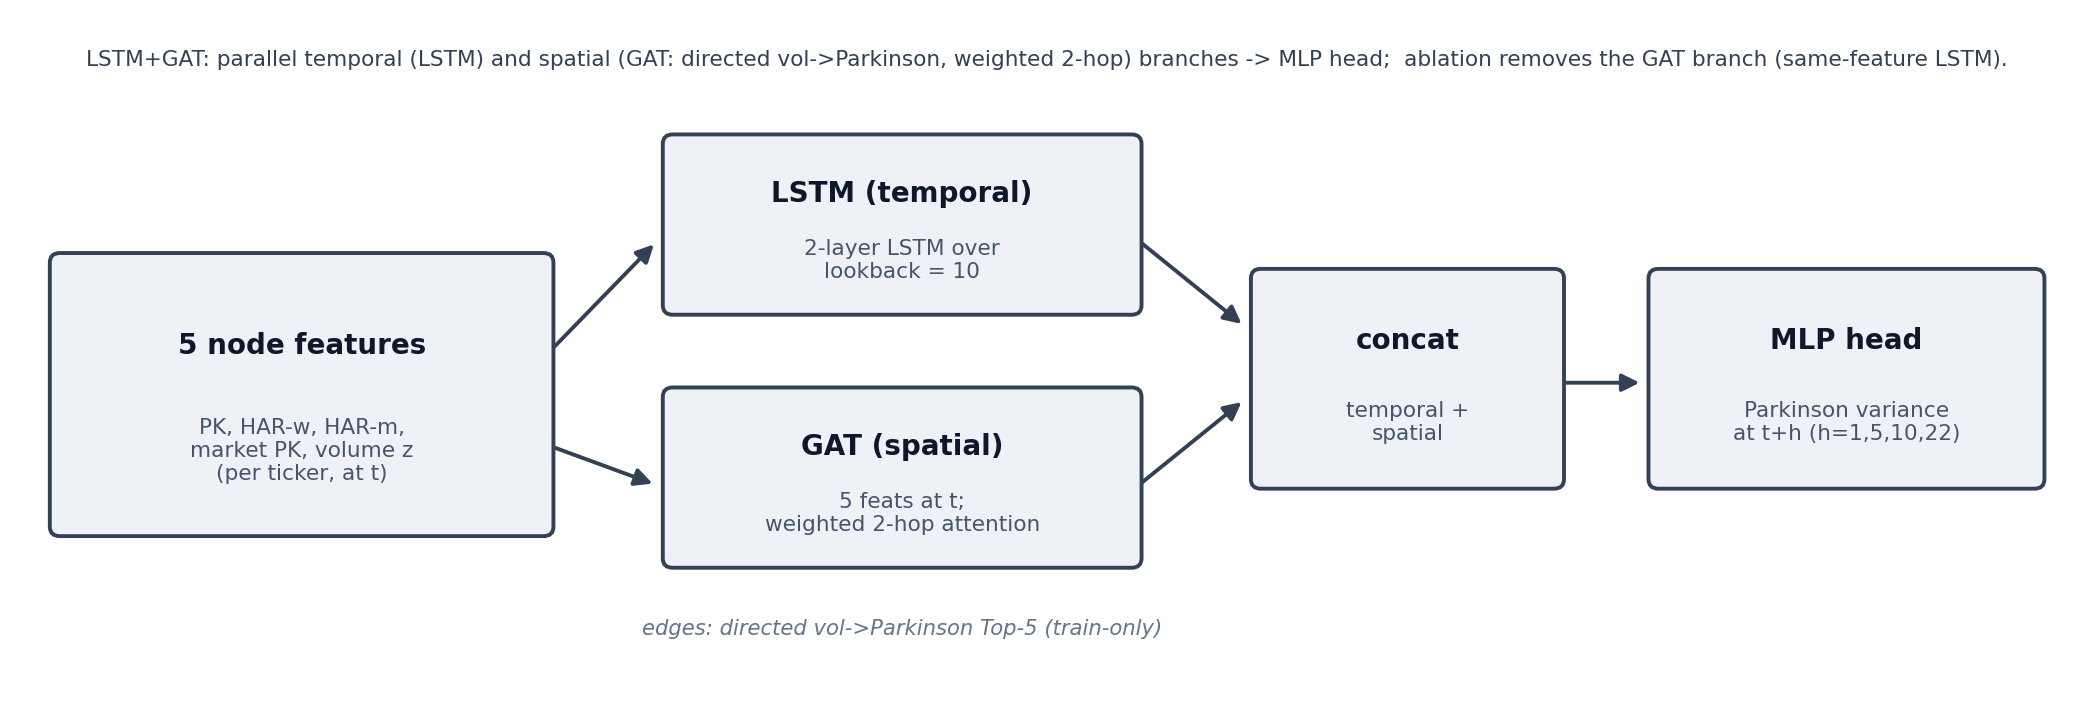
\includegraphics[width=\textwidth]{diagrams/soict_harlstmgat.png}
\caption{LSTM+GAT: a per-node LSTM temporal branch and a GAT spatial branch (directed volume$\to$Parkinson
Top-5 weighted two-hop attention) are concatenated into an MLP head; the leave-one-out comparison removes the
GAT branch to give the same-feature LSTM.}
\label{fig:arch}
\end{figure}

\section{Data}
Two panels are used with the Parkinson target: \textbf{VN30} (primary) and \textbf{VN100} (vnstock). Both use the masked panel of Sec.~3 with the five features, a single chronological
split and per-ticker standardization fit on training rows only.

\section{Experiments}
We compare HAR-X, the five-feature LSTM and the five-feature LSTM+GAT (directed volume$\to$Parkinson weighted
two-hop) on VN30 and VN100 over the masked panel at horizons $\{1,5,10,22\}$, reporting all
five metrics and the two targeted date-clustered DM contrasts (LSTM vs HAR-X, LSTM+GAT vs LSTM).

\section{Results}
Point-error metrics are scaled (MSE $\times10^{-7}$, RMSE $\times10^{-4}$, MAE $\times10^{-4}$); QLIKE and
$R^2$ unscaled. For the learned models each value is the mean of the seed-level metrics over five seeds; the
QLIKE column additionally reports the per-seed standard deviation ($\pm$). HAR-X and GARCH are deterministic.
All values are read from \texttt{results/masked\_rich\_floor1e2/}. Row order is
HAR-X $\to$ GARCH $\to$ LSTM $\to$ LSTM+GAT. Tables~\ref{tab:vn100} and~\ref{tab:vn30} report all five metrics;
Table~\ref{tab:dm} reports the two targeted date-clustered DM contrasts on QLIKE and MAE. The primary horizons
$h1$/$h5$ appear first; the extended horizons $h10$/$h22$ appear in the lower block of each table.

\begin{table}[t]
\centering
\caption{VN100 (46{,}308 masked obs over 454 test dates at $h1$; learned models: seed mean, QLIKE
$\pm$~per-seed std). Lower is better for MSE/RMSE/MAE/QLIKE, higher for $R^2$. $^{\dagger}$~marks metrics where LSTM+GAT improves over the no-graph LSTM. MSE $\times10^{-7}$, RMSE $\times10^{-4}$, MAE $\times10^{-4}$.}
\label{tab:vn100}
\footnotesize
\setlength{\tabcolsep}{5pt}
\begin{tabular}{llccccc}
\toprule
$h$ & Model & MSE & RMSE & MAE & QLIKE & $R^2$ \\
\midrule
1  & HAR-X    & \textbf{2.367} & \textbf{4.865} & 2.898 & \textbf{0.5115} & \textbf{0.2236} \\
1  & GARCH    & 3.816 & 6.178 & 4.538 & 0.7577 & -0.2519 \\
1  & LSTM     & 2.386 & 4.885 & 2.774 & 0.6229\,$\pm$.074 & 0.2172 \\
1  & LSTM+GAT & 2.371$^{\dagger}$ & 4.869$^{\dagger}$ & \textbf{2.773}$^{\dagger}$ & 0.5504\,$\pm$.020$^{\dagger}$ & 0.2224$^{\dagger}$ \\
\midrule
5  & HAR-X    & \textbf{2.606} & \textbf{5.104} & 3.160 & \textbf{0.5633} & \textbf{0.1466} \\
5  & GARCH    & 3.814 & 6.176 & 4.546 & 0.7420 & -0.2493 \\
5  & LSTM     & 2.649 & 5.147 & 3.142 & 0.6021\,$\pm$.039 & 0.1324 \\
5  & LSTM+GAT & 2.634$^{\dagger}$ & 5.132$^{\dagger}$ & \textbf{3.126}$^{\dagger}$ & 0.5759\,$\pm$.012$^{\dagger}$ & 0.1373$^{\dagger}$ \\
\midrule
\multicolumn{7}{l}{\emph{Extended horizons}}\\
10 & HAR-X    & \textbf{2.754} & \textbf{5.248} & 3.306 & \textbf{0.6023} & \textbf{0.0978} \\
10 & GARCH    & 3.891 & 6.238 & 4.582 & 0.7605 & -0.2745 \\
10 & LSTM     & 2.796 & 5.288 & \textbf{3.297} & 0.6100\,$\pm$.008 & 0.0842 \\
10 & LSTM+GAT & 2.812 & 5.303 & 3.342 & 0.6103\,$\pm$.003 & 0.0789 \\
\midrule
22 & HAR-X    & \textbf{2.891} & \textbf{5.377} & \textbf{3.486} & \textbf{0.6405} & \textbf{0.0544} \\
22 & GARCH    & 3.854 & 6.208 & 4.568 & 0.7450 & -0.2603 \\
22 & LSTM     & 2.988 & 5.466 & 3.507 & 0.6525\,$\pm$.001 & 0.0229 \\
22 & LSTM+GAT & 3.029 & 5.504 & 3.600 & 0.6576\,$\pm$.002 & 0.0093 \\
\bottomrule
\end{tabular}
\end{table}

\begin{table}[t]
\centering
\caption{VN30 (10{,}106 masked obs over 326 test dates at $h1$; learned: seed mean, QLIKE $\pm$~per-seed std). $^{\dagger}$~as in Table~1. Same scaling as
Table~\ref{tab:vn100}.}
\label{tab:vn30}
\footnotesize
\setlength{\tabcolsep}{5pt}
\begin{tabular}{llccccc}
\toprule
$h$ & Model & MSE & RMSE & MAE & QLIKE & $R^2$ \\
\midrule
1  & HAR-X    & \textbf{1.927} & \textbf{4.389} & 2.389 & \textbf{0.5159} & \textbf{0.2308} \\
1  & GARCH    & 2.788 & 5.280 & 3.480 & 0.7954 & -0.1129 \\
1  & LSTM     & 1.931 & 4.395 & \textbf{2.352} & 0.7037\,$\pm$.054 & 0.2290 \\
1  & LSTM+GAT & 1.927$^{\dagger}$ & 4.390$^{\dagger}$ & 2.379 & 0.6602\,$\pm$.064$^{\dagger}$ & 0.2305$^{\dagger}$ \\
\midrule
5  & HAR-X    & \textbf{2.139} & \textbf{4.625} & \textbf{2.583} & \textbf{0.5965} & \textbf{0.1497} \\
5  & GARCH    & 2.783 & 5.276 & 3.489 & 0.7859 & -0.1065 \\
5  & LSTM     & 2.158 & 4.645 & 2.636 & 0.6595\,$\pm$.043 & 0.1422 \\
5  & LSTM+GAT & 2.148$^{\dagger}$ & 4.635$^{\dagger}$ & 2.596$^{\dagger}$ & 0.6491\,$\pm$.027$^{\dagger}$ & 0.1461$^{\dagger}$ \\
\midrule
\multicolumn{7}{l}{\emph{Extended horizons}}\\
10 & HAR-X    & \textbf{2.301} & \textbf{4.797} & \textbf{2.733} & \textbf{0.6428} & \textbf{0.1028} \\
10 & GARCH    & 2.829 & 5.319 & 3.508 & 0.7774 & -0.1029 \\
10 & LSTM     & 2.313 & 4.809 & 2.742 & 0.6687\,$\pm$.015 & 0.0984 \\
10 & LSTM+GAT & 2.325 & 4.822 & 2.749 & 0.6672\,$\pm$.029$^{\dagger}$ & 0.0935 \\
\midrule
22 & HAR-X    & \textbf{2.272} & \textbf{4.766} & \textbf{2.785} & \textbf{0.6422} & \textbf{0.0723} \\
22 & GARCH    & 2.719 & 5.214 & 3.437 & 0.7452 & -0.1102 \\
22 & LSTM     & 2.376 & 4.874 & 2.868 & 0.6636\,$\pm$.013 & 0.0299 \\
22 & LSTM+GAT & 2.379 & 4.878 & 2.889 & 0.6527\,$\pm$.003$^{\dagger}$ & 0.0285 \\
\bottomrule
\end{tabular}
\end{table}

\begin{table}[t]
\centering
\caption{Targeted date-clustered DM contrasts on the 5-seed ensemble forecast ($p$-value; favoured model in parentheses; bold if $p<0.05$; unadjusted).
H=HAR-X, L=LSTM, G=LSTM+GAT, on QLIKE and MAE.}
\label{tab:dm}
\footnotesize
\setlength{\tabcolsep}{5pt}
\begin{tabular}{ll cc cc}
\toprule
& & \multicolumn{2}{c}{LSTM vs HAR-X} & \multicolumn{2}{c}{LSTM+GAT vs LSTM} \\
\cmidrule(lr){3-4}\cmidrule(lr){5-6}
Panel & $h$ & QLIKE & MAE & QLIKE & MAE \\
\midrule
VN100 & 1  & \textbf{.001 (H)} & \textbf{$<$.001 (L)} & \textbf{$<$.001 (G)} & .542 (L) \\
VN100 & 5  & .402 (H) & .077 (L) & \textbf{$<$.001 (G)} & \textbf{$<$.001 (G)} \\
VN100 & 10 & .730 (H) & .523 (L) & .453 (L) & \textbf{$<$.001 (L)} \\
VN100 & 22 & .407 (H) & .618 (H) & .140 (L) & \textbf{$<$.001 (L)} \\
\midrule
VN30 & 1  & \textbf{$<$.001 (H)} & \textbf{.003 (L)} & \textbf{$<$.001 (G)} & \textbf{$<$.001 (L)} \\
VN30 & 5  & .122 (H) & \textbf{$<$.001 (H)} & .280 (L) & \textbf{$<$.001 (G)} \\
VN30 & 10 & .249 (H) & .614 (H) & .162 (G) & .331 (L) \\
VN30 & 22 & .520 (H) & .061 (H) & .625 (G) & \textbf{$<$.001 (L)} \\
\bottomrule
\end{tabular}
\end{table}

\textbf{Short-horizon results ($h1$, $h5$).} HAR-X has the lowest QLIKE in all four short-horizon cells, well
below the seed-mean QLIKE of the learned models. At VN100 $h1$ the LSTM+GAT has the lowest MAE, while HAR-X has the lowest MSE, RMSE and $R^2$; the
LSTM+GAT has a higher QLIKE than HAR-X (seed mean $0.5504$ vs $0.5115$). By DM the deep models have a lower
MAE than HAR-X ($p<0.001$) and the LSTM+GAT a significantly lower QLIKE than the no-graph LSTM ($p<0.001$). At
VN100 $h5$ HAR-X has the lowest QLIKE and the LSTM+GAT the lowest MAE; the LSTM+GAT again has a lower QLIKE than
the LSTM ($p<0.001$). At VN30 $h1$ HAR-X has the lowest QLIKE ($0.5159$, against deep seed means of
$0.66$--$0.70$) and the LSTM the lowest MAE ($p=0.003$ vs HAR-X); the LSTM+GAT has a lower QLIKE than the
no-graph LSTM ($p<0.001$). At VN30 $h5$ HAR-X has the lowest value on all five metrics and the graph's QLIKE
advantage over the LSTM is not significant ($p=0.28$). The per-seed QLIKE standard deviation of the learned
models ($0.02$--$0.07$) is comparable to the graph-vs-LSTM gap, so this is an ensemble-level effect within seed
noise.

\textbf{Extended-horizon results ($h10$, $h22$).} HAR-X has the lowest MSE, RMSE, QLIKE and $R^2$ on both
panels at both horizons; the LSTM has the lowest MAE at VN100 $h10$, and HAR-X the lowest MAE in the other
extended-horizon cells. By DM the LSTM+GAT-vs-LSTM QLIKE difference is not significant at $h10$ or $h22$ on
either panel, and no learned model has a significantly lower QLIKE than HAR-X.

\textbf{GARCH benchmark.} GARCH(1,1) has a higher MSE, RMSE, MAE and QLIKE and a lower $R^2$ than HAR-X at
every horizon on both panels, with a negative $R^2$ on both; its QLIKE is higher than HAR-X's under the
date-clustered DM test in all eight cells ($p<0.001$, except VN30 $h22$ where $p=0.001$). GARCH is a frozen-train forecast: a single conditional-variance path is projected from the end of training (persistence capped at 0.999 by variance targeting), so it cannot adapt to the level shifts that HAR-X re-estimates each day, and its error is correspondingly higher.

\textbf{Per-metric ranking.} No single metric determines the ordering, so all five are reported with equal
weight: HAR-X has the lowest QLIKE at every horizon on both panels, with no learned model significantly lower
at any horizon; the deep and graph models have the lowest point error (MAE) at some short horizons on VN100;
and HAR-X has the lowest MSE and RMSE at every horizon.

\textbf{Cross-market check (S\&P 500, exploratory).} As a preliminary out-of-sample check on a larger market, the same masked panel and five features were applied to S\&P 500 constituents (442 nodes, 1{,}624 test dates) with a single seed; Table~\ref{tab:sp500} reports all five metrics. In contrast to the Vietnamese panels, the deep models attain the lowest point error (MSE, RMSE, MAE and $R^2$) from $h5$ onward. HAR-X retains the lowest QLIKE at $h5$, $h10$ and $h22$; at $h1$ the LSTM+GAT has a marginally lower QLIKE. Two caveats apply: the run uses a single seed, and the deep models' QLIKE at $h5$--$h22$ is inflated by the per-node positivity floor at the S\&P 500 variance scale, so QLIKE for the deep models on this panel is not yet reliable and a scale-aware floor with multiple seeds is left for future work.

\begin{table}[t]
\centering
\caption{S\&P 500 (exploratory, single seed): the same masked panel and five features as Tables~1--2, 442 nodes, 1{,}624 test dates. Lower is better for MSE/RMSE/MAE/QLIKE, higher for $R^2$; bold = best per horizon. HAR-X is the same five-feature model as in Tables~1--2. GARCH not run on this panel.}
\label{tab:sp500}
\footnotesize
\setlength{\tabcolsep}{5pt}
\begin{tabular}{llccccc}
\toprule
$h$ & Model & MSE & RMSE & MAE & QLIKE & $R^2$ \\
\midrule
1  & HAR-X     & \textbf{6.171} & \textbf{7.856} & \textbf{2.361} & 0.4078 & \textbf{0.3195} \\
   & LSTM     & 6.367 & 7.979 & 2.453 & 0.4110 & 0.2979 \\
   & LSTM+GAT & 6.384 & 7.990 & 2.466 & \textbf{0.4064} & 0.2960 \\
\midrule
5  & HAR-X     & 8.062 & 8.979 & 2.691 & \textbf{0.4303} & 0.1110 \\
   & LSTM     & \textbf{7.850} & \textbf{8.860} & \textbf{2.573} & 1.0433 & \textbf{0.1344} \\
   & LSTM+GAT & 7.902 & 8.890 & 2.637 & 0.7907 & 0.1287 \\
\midrule
10 & HAR-X     & 8.948 & 9.459 & 2.842 & \textbf{0.4775} & 0.0153 \\
   & LSTM     & 8.505 & 9.222 & 2.767 & 0.8276 & 0.0640 \\
   & LSTM+GAT & \textbf{8.497} & \textbf{9.218} & \textbf{2.701} & 1.0110 & \textbf{0.0650} \\
\midrule
22 & HAR-X     & 9.623 & 9.810 & 2.983 & \textbf{0.6150} & -0.0576 \\
   & LSTM     & 9.399 & 9.695 & 3.259 & 0.8515 & -0.0330 \\
   & LSTM+GAT & \textbf{9.172} & \textbf{9.577} & \textbf{2.952} & 1.3198 & \textbf{-0.0080} \\
\bottomrule
\end{tabular}
\end{table}

\textbf{Output parameterization and QLIKE stability (robustness).} The output parameterization used in the main tables --- a standardized target with a linear output and a relative floor of $10^{-2}$ times the per-node training mean --- was fixed before this investigation. As a robustness check we varied only the deep model's output mapping. Replacing the standardized target with a node-scaled ratio (the model predicts $y_t/\bar{y}_i$ and reconstructs the forecast as the ratio times the training-period node mean) reduces the five-seed QLIKE standard deviation from $0.043$ to $0.005$ (VN30) and from $0.039$ to $0.004$ (VN100) with the same linear output and floor; a positive-by-construction link (exponential or softplus) provides smaller additional improvements and removes the floor. No statistically significant QLIKE difference was detected between the exponential and softplus links at the 5\% level after bias-matched initialization. Table~\ref{tab:robust} reports the five-seed QLIKE for the four configurations.

\begin{table}[t]
\centering
\caption{Output-parameterization robustness (LSTM, $h5$, 5 seeds): QLIKE mean$\pm$std. A: z-score $+$ linear $+$ floor (original); B: ratio $+$ linear $+$ floor; C: ratio $+$ exp (no floor); D: ratio $+$ softplus (no floor). HAR-X QLIKE is 0.5962 (VN30) and 0.5694 (VN100).}
\label{tab:robust}
\footnotesize
\setlength{\tabcolsep}{5pt}
\begin{tabular}{lcccc}
\toprule
Panel & A & B & C & D \\
\midrule
VN30  & $0.660\pm0.043$ & $0.613\pm0.005$ & $0.610\pm0.002$ & $0.610\pm0.003$ \\
VN100 & $0.602\pm0.039$ & $0.572\pm0.004$ & $0.573\pm0.003$ & $0.576\pm0.007$ \\
\bottomrule
\end{tabular}
\end{table}

\textbf{Common-floor sensitivity.} Because the main tables pre-floor HAR-X at the relative floor before the metric, we re-score every model from raw forecasts under a single common floor applied identically to all models, using either the relative floor or a fixed $10^{-8}$ floor. Under both policies fewer than $0.01\%$ of forecasts are clipped, and at $h5$, $h10$ and $h22$ the QLIKE values and the deep-vs-HAR-X DM outcome are identical. Only $h1$ is floor-sensitive, and the sensitivity is on the HAR-X side: extreme $h1$ QLIKE values arose from a very small number of non-positive or near-zero forecasts produced by the unconstrained linear output and subsequently mapped to a tight numerical floor; the positive-by-construction ratio-exp parameterization removed this sensitivity. At $h1$, the ratio-exp deep model obtained a lower mean QLIKE than HAR-X under the relative-floor policy, but no statistically significant difference was detected (VN100 $p=0.24$, VN30 $p=0.57$). These configurations were identified after observing QLIKE on the same test set, so they are reported as a robustness result and as a pre-specified candidate for a future out-of-sample or walk-forward evaluation, not as a replacement for the main-table specification.

\section{Discussion}\label{sec:disc}
No learned model has a significantly lower QLIKE than HAR-X at any horizon under the date-clustered DM test,
and HAR-X has the lowest QLIKE seed-mean in every cell on both panels. At $h1$ the deep models have the lowest
MAE on VN100 (LSTM vs HAR-X, $p<0.001$), and the LSTM+GAT has a significantly lower QLIKE than the same-feature
no-graph LSTM at VN30 $h1$, VN100 $h1$ and VN100 $h5$; this graph effect is absent at VN30 $h5$ and at the
longer horizons. Because the per-seed QLIKE standard deviation of the learned models ($0.02$--$0.07$) is of the
same order as these graph-vs-LSTM differences, and the DM test is computed on the five-seed ensemble forecast,
the graph effect is best read as an ensemble-level regularity rather than a robust per-seed improvement. At
$h10$ and $h22$ HAR-X has the lowest MSE, RMSE, QLIKE and $R^2$. The ranking is metric- and horizon-dependent,
which is why all five metrics are reported with equal weight. The date-clustered DM test matters for these
conclusions: a naive per-observation test on this cross-sectionally dependent panel inflates the statistic by
roughly the square root of the number of stocks, so a difference that is not significant per date can appear
significant per observation. \textbf{Multiplicity.} We report per-metric DM contrasts without a
multiple-comparison correction; the headline conclusion is a set of \emph{null} results (no learned model
significantly beats HAR-X on QLIKE), which a correction would only reinforce, while the significant
graph-vs-LSTM contrasts should be read as unadjusted exploratory findings. \textbf{Capacity.} The LSTM+GAT
adds a graph branch and its parameters to the no-graph LSTM, so the leave-one-out contrast measures the effect
of adding the implemented graph branch, not of graph structure at matched capacity.

\section{Conclusion}
For daily Parkinson-variance forecasting on the Vietnamese market, evaluated with the same features, the same
masked panel and the same date-clustered Diebold--Mariano inference, no learned model has a significantly lower
QLIKE than HAR-X at any horizon, and HAR-X has the lowest QLIKE seed-mean in every cell on both panels. At the
short horizons ($h1$, $h5$) the deep models have the lowest MAE on VN100, and the directed volume$\to$Parkinson
weighted graph gives the LSTM+GAT a significantly lower QLIKE than the same-feature no-graph LSTM at VN30 $h1$,
VN100 $h1$ and VN100 $h5$ --- an ensemble-level difference of the same order as the learned models' per-seed
QLIKE dispersion, and absent at VN30 $h5$; at the extended horizons ($h10$, $h22$) HAR-X has the lowest MSE,
RMSE, QLIKE and $R^2$, and the graph's QLIKE difference from the no-graph LSTM is not significant. The ranking
is metric- and horizon-dependent, so all five metrics are reported with equal weight.

\begin{thebibliography}{99}
\bibitem{corsi2009} Corsi, F.: A simple approximate long-memory model of realized volatility. J. Financial Econometrics \textbf{7}(2), 174--196 (2009)
\bibitem{parkinson1980} Parkinson, M.: The extreme value method for estimating the variance of the rate of return. J. Business \textbf{53}(1), 61--65 (1980)
\bibitem{lstm1997} Hochreiter, S., Schmidhuber, J.: Long short-term memory. Neural Computation \textbf{9}(8), 1735--1780 (1997)
\bibitem{gat2018} Veli\v{c}kovi\'c, P., et al.: Graph attention networks. In: ICLR (2018)
\bibitem{dm1995} Diebold, F.X., Mariano, R.S.: Comparing predictive accuracy. J. Business \& Economic Statistics \textbf{13}(3), 253--263 (1995)
\bibitem{hln1997} Harvey, D., Leybourne, S., Newbold, P.: Testing the equality of prediction mean squared errors. Int. J. Forecasting \textbf{13}(2), 281--291 (1997)
\bibitem{patton2011} Patton, A.J.: Volatility forecast comparison using imperfect volatility proxies. J. Econometrics \textbf{160}(1), 246--256 (2011)
\bibitem{harq2016} Bollerslev, T., Patton, A.J., Quaedvlieg, R.: Exploiting the errors: a simple approach for improved volatility forecasting. J. Econometrics \textbf{192}(1), 1--18 (2016)
\bibitem{chen2022} Chen, Q., Robert, C.-Y.: Multivariate realized volatility forecasting with graph neural network. In: ACM ICAIF (2022). arXiv:2112.09015
\bibitem{gnnhar2025} Zhang, C., Pu, X., Cucuringu, M., Dong, X.: Forecasting realized volatility with spillover effects: perspectives from graph neural networks (2025). arXiv:2308.01419
\bibitem{dy2012} Diebold, F.X., Yilmaz, K.: Better to give than to receive: predictive directional measurement of volatility spillovers. Int. J. Forecasting \textbf{28}(1), 57--66 (2012)
\bibitem{audrino2025} Audrino, F., Chassot, J.: HARd to beat: the overlooked impact of rolling windows in the era of machine learning. Int. J. Forecasting (2025). arXiv:2406.08041
\end{thebibliography}

\end{document}
